\documentclass{beamer}
\usepackage{scuwqt}
\usepackage{booktabs}
\usepackage{mathtools}
\usepackage{dzg-macros}
\usepackage{tikzit}
\usepackage{dynkin-diagrams}

\setlength\parindent{2em}
\renewcommand{\arraystretch}{1.5}
%=========================================================
\title{Moduli of Coble Surfaces}
\author{D. Zack Garza}
\institute{NCTS}
\date{\today}
\setlength{\parindent}{2em}

\begin{document}
{

\begin{frame}
  \titlepage
\end{frame}
%=========================================================
{
    \usebackgroundtemplate{
        \tikz\node[at=(current page.west), yshift=-3cm]  {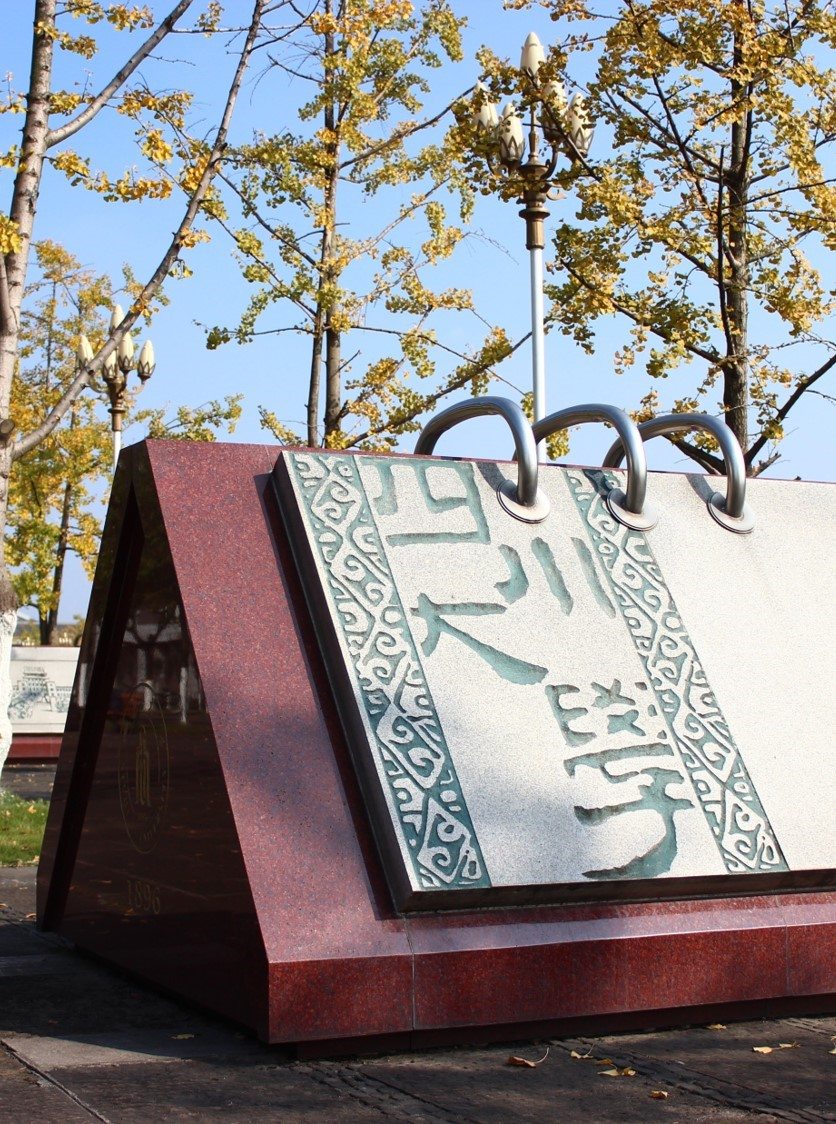
\includegraphics[width=0.5\paperwidth,height=\paperheight]{contents.jpg}};
    }

\begin{frame}

  \hfill 
  \begin{minipage}[t]{.4\textwidth} 
    \tableofcontents 
  \end{minipage}
\end{frame}}
%=========================================================

\section{Introduction}
\subsection{Moduli of Surfaces}

\begin{frame}
\frametitle{Introduction}
\begin{itemize}
\item K3 surface: \quad\hspace{0.6em} $q(X) \coloneqq h^1(\mathcal{O}_X) = 0$ and $\omega_X \cong \mathcal{O}_X$.
\item Enriques surface:  $q(X) = 0$ and $\omega_X \neq \mathcal{O}_X$ but $\omega_X^2 \cong \mathcal{O}_X$.
\item Coble surface: \hspace{1em} $q(X) = 0$, $h^0(\omega_X^{-1}) = 0$ but $h^0(\omega_X^{-2}) > 0$.
\end{itemize}
\vspace{1em}
\begin{centering}
{
\small
\begin{tabular}{l|llllll}
	Surface 	& $\mathrm{ord}(K_X)$ & $\kappa(X)$ 	& $\mathrm{Pic}(X)/\mathrm{tors}$ & $h^{2, 0}$ 
		& $h^{1,1}$ & $h^{0, 2}$ \\ \hline
	K3 			& $1$ & $0$ 			& $L_{K3} \coloneqq U^3 \oplus E_8^2$ 
		& $1$ & $20$ & $1$ \\
	Enriques 	& $2$ & $0$ 			& $L_{En} \coloneqq U \oplus E_8$ 
		& $0$ & $10$ & $0$ \\
	Coble 		& $\infty$ & $-\infty$ 		& $L_{Co} \coloneqq \gens{-1} \oplus U \oplus E_8$
		& $0$ & $11$ & $0$ \\
\end{tabular}
}
\end{centering}
\newline
{\small
\newline
Here $\gens{-1}$ is generated by $K_X$ where $K_X^2 = -1$.
}
\end{frame}
%=========================================================
\begin{frame}\frametitle{TBD}
{
\[
\tiny 
G_U = \begin{pmatrix} 0 & 1 \\ 1 & 0 \end{pmatrix}, \qquad
G_{E_8}
=
\begin{pmatrix}
 -2 &  0 & 1 &  0 &  0 &  0 &  0 &  0 \\
 0 &  -2 &  0 & 1 &  0 &  0 &  0 &  0 \\
1 &  0 &  -2 & 1 &  0 &  0 &  0 &  0 \\
 0 & 1 & 1 &  -2 & 1 &  0 &  0 &  0 \\
 0 &  0 &  0 & 1 &  -2 & 1 &  0 &  0 \\
 0 &  0 &  0 &  0 & 1 &  -2 & 1 &  0 \\
 0 &  0 &  0 &  0 &  0 & 1 &  -2 & 1 \\
 0 &  0 &  0 &  0 &  0 &  0 & 1 &  -2
\end{pmatrix}.
\]
}

\[
\dynkin[edge length=1, root radius=0.1cm,labels={e, f}]{A}{xx}
\qquad
\dynkin[edge length=1, root radius=0.1cm, labels={\alpha_1,\alpha_2,\alpha_3,\alpha_4,\alpha_5,\alpha_6,\alpha_7,\alpha_8}]{E}{oooooooo},
\qquad
\]
\begin{align*}
\dynkin[edge length=0.5, root radius=0.1cm]{A}{x}: v^2 = 0, \qquad 
\dynkin[edge length=0.5, root radius=0.1cm]{A}{o}: v^2 = -2, \qquad
\dynkin[edge length=0.5, root radius=0.1cm]{A}{1}: v^2 = -4
\end{align*}
\end{frame}
%=========================================================
\begin{frame}
\frametitle{TBD}


If $G\actson L$, define 
\[
L^G \da \ts{v\in L \st G.v = v} \leq L, \qquad L_G \da (L^G)^{\perp L}
\]

\begin{itemize}

\item $Y$ Enriques $\implies \exists X\to Y$ its universal cover by a K3.
\item $\pi_1(Y) = \gens{\iota_{\En}} \cong \ZZ/2\ZZ$ 
is a \textbf{nonsymplectic involution}: 
\[
\iota_{\En}(\sigma_X) = -\sigma_X \quad\text{where}\quad H^{2, 0}(X) = \CC\sigma_X
.\]

\item Yields 
\[
S_{\En} \coloneqq L_{K3}^{\gens{\iota_{\En}}} \cong L_{\En}(2) = U(2) \oplus E_8(2)
.\]

\item \cite{Nik79}: if $\iota\actson X$ is a nonsymplectic involution on a K3 surface, there are 75 possibilities for 
\[
S(\iota) \da \lkt^{\gens{\iota}}\quad\text{and}\quad T(\iota) \da S^{\perp \lkt}
.\]

\end{itemize}





\end{frame}
%=========================================================
\begin{frame}\frametitle{TBD}
\begin{center}
\begin{figure}[H]
\centering
\includegraphics[width=0.95\textwidth]{/home/dzack/.pandoc/figures/rendered/nikulin_lattice_pyramid}
\caption{$S_{\dP} = (2,2,0), S_{\En} = (10, 10, 0), S_{\Co} = (11, 11, 1)$.}
\end{figure}
\end{center}

\end{frame}
%=========================================================
\begin{frame}\frametitle{TBD}
For any lattice $T$ of signature $(2, n)$, there is a \textit{period domain} classifying Hodge structures of type $T$, a connected component of
\[
\Omega_T \da \ts{v\in \PP(T \otimes_\ZZ \CC) \st v^2 = 0, \bar{v}\cdot v > 0} = D_T \disjoint \overline{D}_T
.\]
Always a Type \IV Hermitian symmetric domain.
When $T$ is of geometric origin\footnote{e.g. $T = S^{\perp \lkt}$ for $S \injects \Pic(X)$ with $X$ a K3 surface.} and $\Gamma_T \leq \Orth(T)$ the monodromy group of the corresponding \textrm{ZVHS}, $\exists$ a moduli space $S$-polarized K3 surfaces
\[
F_T \da \dcosetl{\Gamma_T}{D_T}
.\]
\end{frame}
%=========================================================
\begin{frame}\frametitle{TBD}
Examples:
{\tiny \begin{center}
\begin{tabular}{l|ll|ll|l}
	$\mcm$ & $S$ & $T$ & $S'$ & $T'$ & $\Gamma_T$ \\ \hline
	$F_{2d}$\cite{Sca87, Laz16, AET23}
		& $\gens{2d}$
		& $\gens{-2d} \oplus U^2 \oplus E_8^2$
		& $\I_{1,0}(2d)$
		& $\I_{0,1}(2d) \oplus \II_{2,18}$ 
		& $\Orth^+(T) \intersect \tilde{\Orth}(T)$ \\

	$F_{\mathrm{ell}}$\cite{ABE22}
		& $U$
		& $U^2 \oplus E_8^2$
		& $\II_{1,1}$
		& $\II_{2,18}$ 
		& $\Orth^+(T) \intersect \tilde{\Orth}(T)$ \\

	$F_{(2,2,0)}$\cite{AE22}
		& $U(2)$
		& $U \oplus U(2) \oplus E_8^2$
		& $\II_{1,1}(2)$
		& $\II_{1,1}(2) \oplus \II_{1,17}$ 
		& $\Orth^+(T) \intersect \tilde{\Orth}(T)$ \\

	$F_{\En}$\cite{Ste95a}
		& $U(2) \oplus E_8(2)$
		& $U \oplus U(2) \oplus E_8(2)$
		& $\II_{1,9}(2)$
		& $\II_{1,1} \oplus \II_{1,9}(2)$ 
		& $\Orth^+(T) \intersect \tilde{\Orth}(T)$ \\
		
	$F_{\En, h}$\cite{Ste95a}
		& $\cdots$
		& $\cdots$
		& $\cdots$
		& $\cdots$
		& $\Orth^+(T) \intersect \Gamma_{T, h}$ \\
\end{tabular}
\end{center}
}

Where
\[
\rho_T: \Orth(T) \to \Orth(A_T), \qquad h \da e + f \in S_{\En} = U(2) \oplus E_8(2)
\]
and
\[
\Gamma_{T, h} = \rho_T\inv\qty{ \rho_S(\Stab_{\Orth(S)}(h) ) },
\qquad
\tilde{\Orth}(T) \da  \rho_T\inv(0)
.\]

% Why $O^+$: $O(T) \actson \Omega_T = D_T \disjoint \bar{D_T}$ does not fix $D_T$

\end{frame}
%=========================================================
\begin{frame}\frametitle{Compactifications}
By \cite{BB66}, $F_T$ is a quasiprojective variety.
When $\mcm$ is a moduli problem with coarse space $F_T$, there are many compactifications:
\[
\gitcpt{\mcm}, \quad
\bbcpt{F_T}, \quad 
\torcpt{F_T}, \quad
\semitorcpt{F_T}, \quad
\ksbacpt{\mcm}\begin{center}\end{center}
\]
\end{frame}
%=========================================================
\begin{frame}\frametitle{TBD}
\ctikzsvg{tikz/compactification_posets_over_BB.tex}
\end{frame}
%=========================================================

\end{document}